% The man-in-the-middle attack (notebook 51, Section 8): (a) without authentication Eve runs one key agreement with
% Alice (pretending to be Bob) and one with Bob (pretending to be Alice), obtains k1 and k2, and relays every message,
% reading or changing it. (b) With a short pre-shared authentication key, every public message carries a tag that only
% a holder of that key can compute; Eve's forged messages are rejected.
\documentclass[tikz,border=6pt]{standalone}
\usepackage{amsmath,amssymb}
\usetikzlibrary{arrows.meta,positioning,calc}
\begin{document}
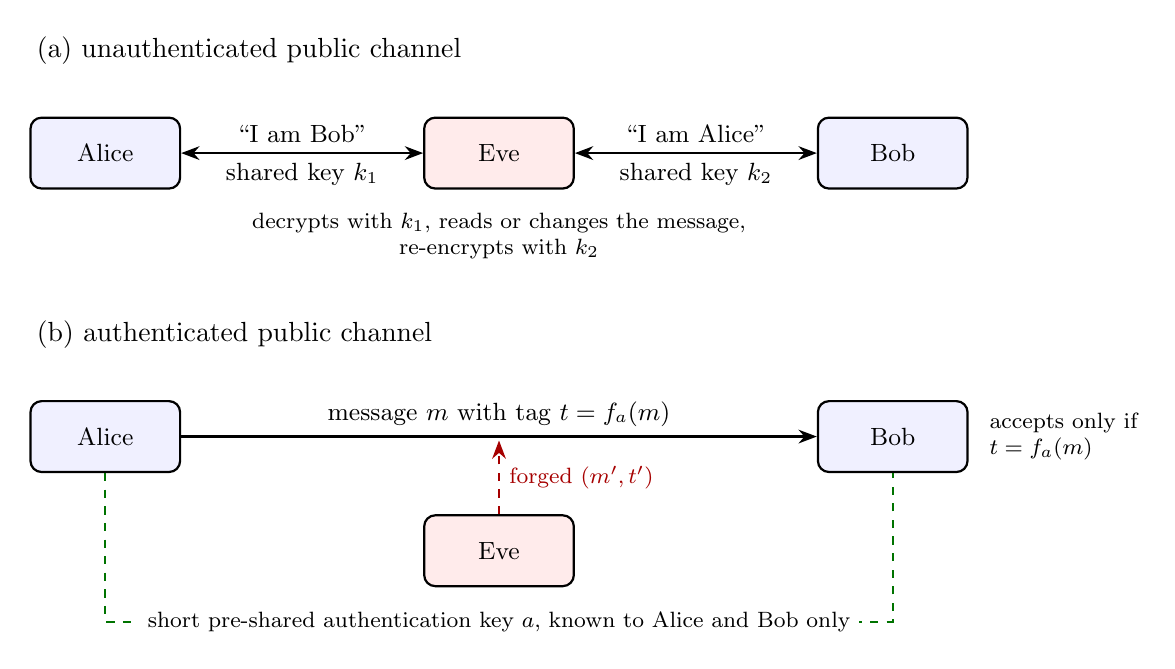
\begin{tikzpicture}[thick, >=Stealth, font=\small,
    party/.style={draw, rounded corners, fill=blue!6, minimum width=1.9cm, minimum height=0.9cm},
    adv/.style={draw, rounded corners, fill=red!8, minimum width=1.9cm, minimum height=0.9cm}]
  % (a) without authentication
  \node[font=\normalsize, anchor=west] at (-1,1.3) {(a) unauthenticated public channel};
  \node[party] (A) at (0,0) {Alice};
  \node[adv] (E) at (5,0) {Eve};
  \node[party] (B) at (10,0) {Bob};
  \draw[<->] (A) -- node[above] {``I am Bob''} node[below] {shared key $k_1$} (E);
  \draw[<->] (E) -- node[above] {``I am Alice''} node[below] {shared key $k_2$} (B);
  \node[font=\footnotesize, align=center] at (5,-1.05)
       {decrypts with $k_1$, reads or changes the message,\\ re-encrypts with $k_2$};
  % (b) with authentication
  \begin{scope}[shift={(0,-3.6)}]
    \node[font=\normalsize, anchor=west] at (-1,1.3) {(b) authenticated public channel};
    \node[party] (A2) at (0,0) {Alice};
    \node[party] (B2) at (10,0) {Bob};
    \draw[->] (A2) -- node[above] {message $m$ with tag $t=f_{a}(m)$} (B2);
    \node[adv] (E2) at (5,-1.45) {Eve};
    \draw[->, dashed, red!65!black] (E2.north) -- (5,-0.05) node[midway, right, font=\footnotesize] {forged $(m',t')$};
    \node[font=\footnotesize, align=left, anchor=west] at (11.1,0) {accepts only if\\ $t=f_{a}(m)$};
    \draw[green!45!black, dashed] (A2.south) -- (0,-2.35) --
      node[fill=white, text=black, font=\footnotesize]
      {short pre-shared authentication key $a$, known to Alice and Bob only}
      (10,-2.35) -- (B2.south);
  \end{scope}
\end{tikzpicture}
\end{document}
